\documentclass[mat1, tisk]{fmfdelo}
% \documentclass[fin1, tisk]{fmfdelo}
% Če pobrišete možnost tisk, bodo povezave obarvane,
% na začetku pa ne bo praznih strani po naslovu, …

%%%%%%%%%%%%%%%%%%%%%%%%%%%%%%%%%%%%%%%%%%%%%%%%%%%%%%%%%%%%%%%%%%%%%%%%%%%%%%%
% METAPODATKI
%%%%%%%%%%%%%%%%%%%%%%%%%%%%%%%%%%%%%%%%%%%%%%%%%%%%%%%%%%%%%%%%%%%%%%%%%%%%%%%

% - vaše ime
\avtor{Tjaž Eržen}

% - naslov dela v slovenščini
\naslov{Paralelizacija grafovskih algoritmov v funkcijskih programskih jezikih}

% - naslov dela v angleščini
\title{Parallelisation of Graph Algorithms in Functional Programming Languages}

% - ime mentorja/mentorice s polnim nazivom:
\mentor{izr.~prof.~dr.~Matija Pretnar}

% - leto diplome
\letnica{2023} 



% - povzetek v slovenščini
%   V povzetku na kratko opišite vsebinske rezultate dela. Sem ne sodi razlaga
%   organizacije dela, torej v katerem razdelku je kaj, pač pa le opis vsebine.
\povzetek{TODO}

% - povzetek v angleščini
\abstract{TODO}

% - klasifikacijske oznake, ločene z vejicami
%   Oznake, ki opisujejo področje dela, so dostopne na strani https://www.ams.org/msc/
\klasifikacija{68R10, 68W10, 68N18, 68N19, 05C85}

% - ključne besede, ki nastopajo v delu, ločene s \sep
\kljucnebesede{TODO}

% - angleški prevod ključnih besed
\keywords{TODO} % angleški prevod ključnih besed

% - angleško-slovenski slovar strokovnih izrazov
\slovar{
\geslo{high performance computing}{Visokozmožnostno računanje}
\geslo{domains}{domene}
\geslo{parallel tasks}{vzporedne naloge}
\geslo{task collections}{zbirke opravil}
\geslo{parallel computation patterns}{vzorci vzporednega računanja}
\geslo{synchronization primitives}{sinhronizacijski mehanizmi}
\geslo{load balancing}{Izravnavanje obremenitve}
\geslo{high-level}{visokonivojski}
\geslo{code wrapper}{programski ovoj}
\geslo{adjaceny list}{seznam sosednosti}
\geslo{shared memory}{skupni pomnilnik}
\geslo{distributed memory}{porazdeljeni pomnilnik}
\geslo{thread race}{dirka podatkov} % TODO: Je to dober prevod?
\geslo{vzajemna izključitev}{mutex}
\geslo{overhead}{dodatna računska obremenitev}
}

% - ime datoteke z viri (vključno s končnico .bib), če uporabljate BibTeX

\literatura{literatura.bib}


%%%%%%%%%%%%%%%%%%%%%%%%%%%%%%%%%%%%%%%%%%%%%%%%%%%%%%%%%%%%%%%%%%%%%%%%%%%%%%%
% DODATNE DEFINICIJE
%%%%%%%%%%%%%%%%%%%%%%%%%%%%%%%%%%%%%%%%%%%%%%%%%%%%%%%%%%%%%%%%%%%%%%%%%%%%%%%

% naložite dodatne pakete, ki jih potrebujete
\usepackage{algpseudocode}  % za psevdokodo
\usepackage{algorithm}      % za algoritme
\usepackage{algorithmicx}
\usepackage{hyperref}
\usepackage{listings}
\usepackage{tikz}
\usepackage{circuitikz}
\usetikzlibrary{shapes,arrows}

\hypersetup{
    colorlinks=true,
    linkcolor=blue,
    filecolor=magenta,
    urlcolor=cyan,
    citecolor=red
}

% Set the font size for all listings
\lstset{basicstyle=\footnotesize\ttfamily}

\algnewcommand\algorithmicto{\textbf{to}}
\algnewcommand\algorithmicin{\textbf{in}}
\algnewcommand\algorithmicforeach{\textbf{for each}}
\algrenewtext{For}[3]{\algorithmicfor\ #1 $\gets$ #2\ \algorithmicto\ #3\ \algorithmicdo}
\algdef{S}[FOR]{ForEach}[2]{\algorithmicforeach\ #1\ \algorithmicin\ #2\ \algorithmicdo}


\floatname{algorithm}{Algoritem}
\renewcommand{\listalgorithmname}{Kazalo algoritmov}

\newcommand{\R}{\mathbb R}
\newcommand{\N}{\mathbb N}
\newcommand{\Z}{\mathbb Z}
\newcommand{\C}{\mathbb C}
\newcommand{\Q}{\mathbb Q}

\lstdefinelanguage{OCaml}{
  keywords={let,rec,if,then,else,module},
  sensitive=true,
  basicstyle=\ttfamily,
  keywordstyle=\bfseries,
  showstringspaces=false,
  morecomment=[s]{(*}{*)},
  morestring=[b]"
}

\lstset{
  language=Caml,
  frame=single,
  numbers=left,
  numberstyle=\tiny,
  stepnumber=1,
  numbersep=5pt,
  tabsize=2,
  breaklines=true,
  prebreak=\raisebox{0ex}[0ex][0ex]{\ensuremath{\hookleftarrow}},
  showtabs=false,
  showspaces=false,
  showstringspaces=false,
  basicstyle=\ttfamily\small,
  identifierstyle=\ttfamily\small,
  commentstyle=\color{gray}\ttfamily\small,
  keywordstyle=\color{blue}\ttfamily\small,
  stringstyle=\color{red}\ttfamily\small
}


%%%%%%%%%%%%%%%%%%%%%%%%%%%%%%%%%%%%%%%%%%%%%%%%%%%%%%%%%%%%%%%%%%%%%%%%%%%%%%%
% ZAČETEK VSEBINE
%%%%%%%%%%%%%%%%%%%%%%%%%%%%%%%%%%%%%%%%%%%%%%%%%%%%%%%%%%%%%%%%%%%%%%%%%%%%%%%

\begin{document}

\section{Uvod}

Grafovski algoritmi so ključni pri modeliranju širokega nabora vsakdanjih problemov: 
Igrajo pomembno vlogo pri modeliranju družbenih ter računalniških omrežjih, z njimi pa se prav tako razrešujejo 
problemi na področjih računalniške komunikacije ter podatkovne analitike. Splošno, z grafi  modeliramo kakršne 
koli odnose med danimi entitetami, vse od računanja razdalj med mesti, pa do računanje vodnega pretoka 
od enega kraja do drugega.

Kot kompleksnost grafov narašča, se povečujejo tudi zahteve za računsko
moč pri njihovem obdelovanju. Čeprav so grafovski algoritmi v osnovi
izračunljivi, lahko obdelava velikih ali zapletenih grafov postane izjemno
zahtevna, tako v smislu časa izvajanja kot porabe pomnilnika.
Načinov za reševanje tega problema je več, pogosto pa je eden izmed možnih načinov pospešitve
programa paralelizacija, s čimer, kot bomo videli, bolje izkoristimo celotno računsko kapaciteto računalnika.
Posledično je paralelizacija tovrstnih algoritmov v zadnjih letih postala tako zanimiva raziskovalna kot
tudi aplikativna tema v računalništvu.

Funkcijski programski jeziki zagotavljajo matematične abstrakcije na višjem nivoju, kot so jih to sposobni navadni
imperativni programski jeziki, kot so na primer \textit{Python}, \textit{C++} in \textit{Java}. 
Ena izmed prednosti funkcijskih programskih jezikov je, da omogočajo deklarativno programiranje, 
kar jih naredi bolj paralelizabilne.

\emph{Funkcijsko programiranje} je računalniški koncept, znotraj katerega programe
pišemo z komponiranjem in apliciranjem matematičnih funkcij. 

\emph{Deklarativni programski jezik} je vrsta programskega jezika, kjer razvijalec opiše kaj naj program stori, 
namesto kako naj to stori. Programi so tipično strukturirani kot nizi deklaracij, ki določajo razmerja in omejitve
med različnimi entitetami znotraj problema. 
Nasprotno, \textbf{imperativni programski jezik} je vrsta programskega jezika, kjer programer navede zaporedje ukazov,
ki naj jih računalnik izvrši za rešitev problema.

Vzporednost na nivoju procesorja je moč doseči na dva načina: 
Tako, da je pomnilnik vsem računalniškim jedrom skupen, ali pa da je pomnilnik \textit{porazdeljen}. 
V tej diplomski nalogi se bom osredotočal zgolj na sisteme s skupnim pomnilnikom ter porazdeljeno procesorsko močjo, 
saj je tovrstne programe tipično manj zahtevno implementirati, kot pa tiste, ki delujejo na porazdeljenem pomnilniku.

Vzporednost na nivoju procesorja je moč doseči na dva načina: 
Tako, da je pomnilnik vsem računalniškim jedrom skupen, ali pa da je pomnilnik \textit{porazdeljen}. 
V tej diplomski nalogi se bom osredotočal zgolj na sisteme s skupnim pomnilnikom ter porazdeljeno procesorsko močjo.
V splošnem je programe na porazdeljenem pomnilniku težje implementirati, saj moramo še dodatno skrbeti za sinhronizacijo
med procesi.

Vse več funkcijskih programskih jezikov, kot so na primer Scala, F\# ter Haskell ima implementirane knjižnice
in ogrodja za paralelizacijo grafovskih algoritmov:
\begin{itemize}
    \item knjižnica \textit{fgl} v Haskellu \cite{haskell_fgl} zagotavlja vzporedne algoritme za najkrajšo pot 
    ter iskanje krepko povezanih komponent.
    \item \textit{GraphX} v Scali \cite{graphx} ponuja implementacijo paralelnega Googlovega PageRank algoritma.
\end{itemize}

Z izdajo različice 5.0.0 leta 2022 je tudi OCaml dobil podporo za paralelno računanje. Zato sem to priložnost 
izkoristil, da svoje računalniške programe pišem v tem funkcijskem jeziku. 
V svoji diplomski naloge se bom tako spustil v tovrstne knjižnice v funkcijskih jezikih, ki že obstajajo, 
pregledal novejše raziskave kar se tiče grafovskih algoritmov v imperativnih jezikih, 
tovrstne ideje poskušal razumeti v kontekstu funkcijskih jezikov ter vse skupaj povezal v preprosto knjižnico v OCamlu.

Ker je OCaml šele nedavno dobil podporo za paralelizacijo, je literatura na to temo omejeno.
Med obstoječimi viri je knjižnica OCaml Multicore \cite{ocaml_multicore_500}, ki se osredotoča na paralelizacijo redkih grafov.
To je narekovalo potrebo po uporabi OCamlove dokumentacije o paralelizaciji \cite{ocaml_paralelisation_documentation} ter
raziskovanju knjižnic, razvitih v drugih funkcijskih jezikih. Za osnovo pri razvoju grafa je bila uporabljena knjižnica,
razvita v Swiftu \cite{functional_swift_graph}, medtem ko so bile za implementacijo grafovskih algoritmov in strukturiranje
knjižnice uporabljene tehnike iz knjižnice Haskell \cite{haskell_fgl}.

\subsection{Kaj lahko od paralelnega programa pričakujemo?}

V praksi od paralelnega programa pričakujemo predvsem višjo hitrost izvajanja v primerjavi s sekvenčnim programom,
kjer se naloge izvajajo zaporedno. Teoretično gledano, zakon Amdahl \cite{amdahl1967} določa omejitve pospešitve,
ki jih lahko dosežemo z paralelizacijo. Čeprav teoretično program s $n$ procesorji lahko doseže do $n$-kratno hitrost,
je treba upoštevati dodatne računske obremenitve, ki nastanejo pri vzpostavitvi paralelnega izvajanja, vključno s
sinhronizacijo procesov, upravljanjem virov in koordinacijo med procesorskimi enotami. Tako lahko v nekaterih primerih,
zlasti pri izvajanju na enem samem jedru, paralelni program postane počasnejši od svojega sekvenčnega ekvivalenta.
Te ugotovitve ilustrira slika \ref{fig:cilj-casovne-zahtevnosti-paralelizacije}, pri čemer je pomembno tudi razmisliti o
optimalnem razporejanju nalog in upravljanju virov za maksimalno izkoristek paralelizacije.

\begin{figure}[h!]
  \centering
  \caption{V našem programu si želimo, da bo čas izvedbe našega programa ujet med spodnjo in zgornjo mejo.}
  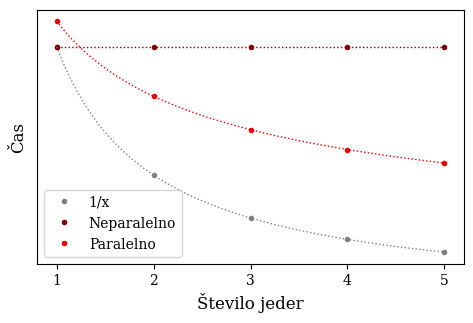
\includegraphics[width=13cm]{slike/cilj-casovne-zahtevnosti-paralelizacije.png}
  \label{fig:cilj-casovne-zahtevnosti-paralelizacije}
\end{figure}

\subsection{Prednosti paralelizacije v funkcijskih programskih jezikih}

\emph{Stranski učinki} so v programiranju kakršen koli odklon med čistimi matematičnimi funkcijami ter našim programom.

Zakaj koncepta funkcijskih programskih jezikov ter paralelizacije tako dobro sovpadata skupaj?
V primerjavi z drugimi vrstami programskih jezikov, kot so na primer imperativni programski jeziki,
so funkcijski programski jeziki bolj primerni za paralelizacijo iz več razlogov 
\cite{parallelisation_advantages_stack_discussion_2023, functional_parallel_graph_rewriting}:

\begin{itemize} \label{itemize:prednosti_funkcijskega_programiranja}
  \item \textbf{Nespremenljivost in odsotnost stranskih učinkov:} 
    Elementarne podatkovne strukture v funkcijskih programskih jezikih običajno nespremenljive, kar za sabo prinese številne
    prednosti, kot so na primer lažje razumevanje in odpravljanje napak, učinkovitost, modularnost 
    ter druge. Vse te lastnosti pa so še posebej pomembne v paralelnem kontekstu, kjer so naloge pogosto razdeljene med
    različne niti ali stroje. Če nam je zagotovljeno, da naša funkcija ne spreminja nobenega skupnega stanja, se
    različni procesi lahko izvajajo vzporedno, ne da bi se pri tem bilo treba ukvarjati s tem, da bi več procesov
    naenkrat posegalo po istem prostoru v pomnilniku, ali z drugimi sinhronizacijskimi težavami.
    Iz praktičnih izkušenj je razvidno, da uporaba spremenljivih podatkovnih struktur v OCamlu, kot sta na primer
    \texttt{Array} in \texttt{reference}, lahko povzroči težave pri pisanju paralelnih programov, saj to zahteva
    dodatno upravljanje sinhronizacije in stanja med procesi.

  \item \textbf{Lažje razumevanje in odpravljanje napak:} 
    Odsotnost stranskih učinkov prav tako olajša razumevanje kode in njeno odpravljanje napak, kar je še posebej
    pomembno pri paralelnem programiranju, kjer je težko slediti stanju programa.

  \item \textbf{Modularnost in ponovna uporabnost:}
    Funkcijsko programiranje spodbuja pisanje majhnih, čistih funkcij, s čimer poskrbimo, da je naša koda bolj 
    modularna in ponovno uporabna. To je lahko velika prednost v paralelnem kontekstu,
    kjer je naloge pogosto treba razbiti na manjše, neodvisne enote, ki se lahko izvajajo vzporedno.

  \item \textbf{Deklarativna narava funkcijskih jezikov:} 
    Funkcijsko programiranje je oblika deklarativnega programiranja, kar pomeni, da opisujete, kaj želimo doseči, 
    ne da bi natančno opisali, kako to doseči. Ta visoka stopnja abstrakcije lahko olajša pisanje paralelne kode, 
    saj se lahko osredotočite na problem, ne da bi se zapletli v podrobnosti paralelnega izvajanja.
\end{itemize}

Ko potrebujem implementacijo določene podatkovne strukture v imperativnem programskem jeziku, kot je na primer
\textit{Python}, je pogosto dovolj, da v splošnem učbeniku najdem njeno implementacijo ter to prepišem.
Razvijalci, ki pa svojo kodo pišejo v funkcijskih programskih jezikih, pa zaradi manjše
razširjenosti funkcijskih programskih jezikov pogosto te sreče nimajo.
Dodatno smo zaradi stroge omejitve odsotnosti stranskih učinkov v funkcijskih jezikih primorani, da se izogibamo
programskim konstruktom, ki pomnilnik spreminjajo, na primer zanka. To pa je v primeru implementacije grafovskih
algoritmov, kjer se moramo npr. sprehoditi po sosedih trenutnega vozlišča, pogosto precej težavno.

Pogosto se zgodi, da podatkovna struktura v imperativnih jezikih nima svojega ekvivalenta v funkcijskih jezikih.
Pri implementaciji različnih podatkovnih struktur, kot je na primer vrsta s prednostjo v poglavju
\ref{section:dijkstra}, mi je bila v veliko pomoč knjiga \cite{okasaki1996}.

V nadaljevanju dokumenta se bom najprej posvetil vprašanju, kako graf v funkcijskih jezikih sploh predstavimo, 
nato pa se bom lotil algoritmov ter podatkovnih struktur na grafih.

\section{Predstavitev grafa v funkcijskih jezikih}

Če hočemo implementirati kakršen koli grafovski algoritem, je prvi korak, da graf sploh predstavimo v našem programu.
Kot smo utemeljili v razdelku \ref{itemize:prednosti_funkcijskega_programiranja}, se grafa lotimo z nespremenljivimi
podatkovnimi strukturami.

Definiral sem tri module: \texttt{Node} ter \texttt{UnweightedGraph} ter \texttt{WeightedGraph}, ki predstavljajo
vozlišče ter graf. V OCamlu modul predstavlja zbirko združenih podatkovnih tipov, funkcij ter drugih modulov v enoto.
Vsak modul ima svojo signaturo, ki predstavlja javni del modula, ter implementacijo, ki predstavlja privatni del modula.
Signatura modula je vmesnik, ki ga uporabnik vidi, implementacija pa je dejanska implementacija funkcij in tipov,
deklariranih v signaturi. To omogoča skrivanje podrobnosti implementacije, ki jih uporabnik ne potrebuje. Abstraktni tipi, kot sta
\texttt{t} in \texttt{elt} v signaturi modula \texttt{Node}, so tisti, katerih implementacijo skrijemo pred uporabnikom.
Na primer, modul \texttt{Node} vključuje funkcije kot so \texttt{create}, \texttt{value} in \texttt{compare}, ter abstraktni
podatkovni tip \texttt{t}, ki predstavlja vozlišče. Na podoben način sem definiral tudi modula \texttt{UnweightedGraph}
ter \texttt{WeightedGraph}, ki predstavljata neutežen ter utežen graf.
Celotna implementacija modulov je na voljo na \href{https://github.com/tjazerzen/parallelisation-of-graph-algorithms-in-functional-programming-languages/blob/master/playground/graph/graph.ml}{tem naslovu},
tu pa predstavim glavno idejo zasnove modulov.

\texttt{Node} je modul, ki predstavlja vozlišče grafa. 
Vsako vozlišče ima svoj identifikator (\texttt{id}) ter celoštevilsko vrednost (\texttt{value}). Pri tem poskrbim, da uporabnik ne 
operira direktno z identifikatorjem vozlišča, temveč preko funkcij, ki so na voljo v tem modulu.
S tem izničimo možnost, da bi na primer uporabnik ustvaril dve vozlišči z istim ID-jem. 
Kot na primer vidimo iz funkcijskega zapisa \texttt{val create : elt -> t}, je za ustvarjanje vozlišča potrebna
zgolj vrednost vozlišča, s katero bomo to vozlišče ustvarili, njegov identifikator pa se bo samodejno povečal.
Podobna logika velja za ostale metode znotraj vseh modulov: Metode sprejmejo ključne argumente, ki jih potrebujejo
za svoje delovanje, vrne pa vrednost abstraktnega tipa v danemu modulu.

\begin{lstlisting}
module Node : sig
  type elt = int
  type t
  val compare_ids : t -> t -> int
  val create : elt -> t
  val value : t -> elt
  val compare : t -> t -> int
  val to_string : t -> string
end = struct
  type elt = int
  type t = { id : int; value : elt }

  let compare_ids node1 node2 = 
    Stdlib.compare node1.id node2.id
  ...
end

module NodeSet = Set.Make (Node)
module NodeMap = Map.Make (Node)

\end{lstlisting}

\texttt{UnweightedGraph} je modul, ki predstavlja neutežen graf. 
Tu sem uporabil OCamlov modul Map (\url{https://ocaml.org/docs/map}) s vozlišči kot ključi ter množicami sosednjih vozlišč
kot vrednostmi. Tako lahko na primer dostopamo do sosedov vozlišča $v$ z uporabo funkcije \texttt{NodeMap.find v graph.edges}.
Poleg tega sem dodal metode, ki bi si jih za graf tipično želeli: Dodajanje ter odvzem
vozlišč in povezav, pridobivanje seznama vseh vozlišč ter povezav, pridobivanje seznama sosedov danega vozlišča
ter druge.

\begin{lstlisting}

module UnweightedGraph : sig
  type elt = int (* node values *)
  type t (* graphs *)

  val empty : directed:bool -> t
  val add_node : Node.t -> t -> t
  val remove_node : Node.t -> t -> t
  val add_edge : Node.t -> Node.t -> t -> t
  val remove_edge : Node.t -> Node.t -> t -> t
  val nodes : t -> Node.t list
  val edges : t -> (Node.t * Node.t) list
  val to_string : t -> string
  val neighbours : Node.t -> t -> Node.t list
  val create_new_graph : num_nodes:int -> num_edges:int -> directed:bool -> t
end = struct
  type elt = int
  type t = {
    edges : NodeSet.t NodeMap.t;
    directed : bool;
  }
  ...
end

\end{lstlisting}

S podobnimi metodami definiram tudi modul \texttt{WeightedGraph}, le da je njegov zapisni
tip enak
\begin{lstlisting}
module WeightedGraph : sig
  type elt = int
  type t
  ...
end = struct
  type elt = int
  type t = {
    edges : float NodeMap.t NodeMap.t; 
    directed : bool
  }
  ...
end
\end{lstlisting}

Modul \texttt{WeightedGraph} se torej od modula \texttt{UnweightedGraph} razlikuje zgolj v tem, da je preslikava, ki
predstavlja povezave, sedaj preslikava, ki vsakemu vozlišču priredi preslikavo, ki njegovim sosedom priredi težo povezave.
Tako kot pri neuteženem grafu, tudi tukaj poskrbim za vse metode, ki bi si jih tipično za graf želeli.

\section{Paralelizacija}

\subsection{Pregled OCamlove knjižnice \textit{Domainslib}} \label{sec:pregled_domainslib}

\href{https://github.com/ocaml-multicore/domainslib}{Domainslib} je sočasna programska knjižnica za OCaml, 
ki nam omogoča paralelizacijo na nivoju procesorja. Ponuja nam razne abstrakcije in orodja za pisanje vzporednih
in sočasnih programov. Zgrajena je na t.i. domenah (ang. domains). To so lahke niti, vgrajene v OCaml.
S prihodom OCamlove različice 5.0.0 je \texttt{Domainslib} postal tudi del standardne knjižnice OCaml.

Tukaj povzamem glavne koncepte Domainsliba, ki jih bom uporabil v svoji diplomski nalogi:

\begin{itemize} \label{itemize:domainslib}
  \item \emph{Domene} (ang. domains) so niti, ki nam zagotavljajo sočasnost v OCaml-u. 
        Po svoji zasnovi so visokonivojske ter imajo nizke stroške dodatne računske obremenitve, kar
        omogoča ustvarjanje velikega števila sočasnih nalog. Domene so definirane znotraj t.i. bazena nalog
        (angl. task pool), znotraj katerega specificiramo število domen, ki jih želimo ustvariti. Nov bazen
        nalog ustvarimo z ukazom ~\texttt{Domainslib.Task.setup\_pool}.
  \item \emph{Paralelne naloge} (ang. parallel tasks): Knjižnica nam ponuja preproste funkcije za ustvarjanje in upravljanje
        z vzporednimi nalogami. Naloge so delovne enote, ki se lahko izvajajo hkrati na različnih domenah.
        Ustvarijo se s funkcijo ~\texttt{Domainslib.Task.async}, na njihovo dokončanje pa se počaka z uporabo
        ~\texttt{Domainslib.Task.await}.
  \item \emph{Zbirke opravil} (ang. task collections): Knjižnica nam ponuja zbirke opravil, ki so podobne paralelnim nalogam, 
        le da lahko v njih shranimo več nalog hkrati. Zbirke opravil so uporabne, kadar želimo ustvariti več nalog hkrati,
        vendar pa ne želimo ustvariti toliko domen, kot je nalog.
  \item \emph{Vzorci vzporednega računanja} (ang. parallel computation patterns), ki so pogosto uporabni pri vzporednem
        programiranju. Na primer, z ukazom \linebreak \texttt{Domainslib.Parallel.For} vzporedno poženemo zanko \texttt{for}.
        Vse to nam precej olajša delo, če lahko večji kos računalniške naloge razdelimo na manjše kose, ki jih lahko
        izvajamo vzporedno že preko vgrajenih funkcij.
  \item \emph{Sinhronizacijski mehanizmi} (ang. synchronization primitives): Knjižnica nam ponuja sinhronizacijske mehanizme,
        ki nam omogočajo sinhronizacijo med domenami. Za to se uporablja modul ~\texttt{Atomic}. Obratno lahko definiramo
        mehanizme za vzajemno izključitev podatkovnih tokov (ang. mutex), ki nam omogočajo, da se določen kos kode
        izvaja samo na eni domeni hkrati. Za to se uporablja modul ~\texttt{Mutex}.
  \item \emph{Izravnavanje obremenitve} (ang. load balancing): Domainslib nam ponuja orodja za izravnavanje obremenitve, 
        ki nam omogočajo, da se obremenitev med domenami porazdeli čim bolj enakomerno.
\end{itemize}

Na splošno knjižnica Domainslib ponastavlja postopek pisanja vzporednih in sočasnih programov v OCamlu. 
Zagotavlja nam visokonivojski (ang. high-level) vmesnik za upravljanje nalog, usklajevanje sinhronizacije in
izkoriščanje vzporednosti, kar olajša izkoriščanje celotnega potenciala večjedrnih procesorjev ter doseganje boljše
zmogljivosti.

Za več informacij in uradno implementacijo knjižnice Domainslib lahko obiščete uraden repozitorij
knjižnice Domainslib na GitHub-u na spletnem naslovu \url{https://github.com/ocaml-multicore/domainslib}.


\subsection{Uvodni primer: Računanje Fibonaccijevih števil}

Čeprav ne gre za grafovski algoritem, je vseeno poučno, da najprej predstavimo osnovne koncepte
paralelizacije na kar se da preprostem primeru. Izbral sem si paralelno računanje Fibonaccijevih števil
(na način, ki terja časovno zahtevnost $O(2^n)$, kot je razvidno iz slike \ref{fig:fib-graph}).
Osnovno idejo problema sem povzel po \cite{parallel_fib_computation} in \cite{multicore_ocaml_article} ter jo prilagodil
za lastne potrebe.

Preprosto funkcijo, ki računa Fibonaccijevo število, lahko zapišemo na zelo preprost način:

\subsubsection{Sekvenčno računanje Fibonaccijevih števil}

\begin{lstlisting}
  let rec fib n =
    if n < 2 then 1
    else fib (n-1) + fib (n-2)
\end{lstlisting}

\begin{figure}[htb]
  \centering
  \begin{tikzpicture}[node distance=2cm]

    % level 0
    \node (n0) at (0,0) {$n$};

    % level 1
    \node (n1) at (-2,-2) {$n-1$};
    \node (n2) at (2,-2) {$n-2$};

    % level 2
    \node (n3) at (-4,-4) {$n-2$};
    \node (n4) at (-1.5,-4) {$n-3$};
    \node (n5) at (1.5,-4) {$n-3$};
    \node (n6) at (4,-4) {$n-4$};

    % level 3
    \node (n7) at (-5.5,-6) {$n-3$};
    \node (n8) at (-3,-6) {$n-4$};
    \node (n9) at (-1,-6) {$n-4$};
    \node (n10) at (0,-6) {...};

    \draw [->] (n0) -- (n1);
    \draw [->] (n0) -- (n2);
    \draw [->] (n1) -- (n3);
    \draw [->] (n1) -- (n4);
    \draw [->] (n2) -- (n5);
    \draw [->] (n2) -- (n6);
    \draw [->] (n3) -- (n7);
    \draw [->] (n3) -- (n8);
    \draw [->] (n4) -- (n9);
    \draw [->] (n4) -- (n10);

  \end{tikzpicture}
  \caption{Ker na vsakem koraku rekurzivno kličemo problema velikosti $n-1$ in $n-2$, se naša rekurzija razveja
  kot skoraj polno dvojiško drevo. Zato je časovna zahtevnost našega algoritma eksponentna (natančna zgornja meja je 
  $O((\frac{1 + \sqrt{5}}{2})^n)$).}
  \label{fig:fib-graph}
\end{figure}


\subsubsection{Paralelno računanje Fibonaccijevih števil}

Zato se seveda vprašamo, kako bi lahko to funkcijo paralelizirali. Očiten odgovor je, da bi lahko paralelno računali
$fib(n-1)$ in $fib(n-2)$ ter to počeli, dokler ne pridemo do baze rekurzije. To lahko predstavimo z grafom, kot je
prikazano na sliki \ref{fig:fib-graph}. Problem, na katerega sem naletel ob empiričnem testiranju svojega programa
je, da je ta način paralelizacije precej neučinkovit, saj tako definirano število paralelnih nalog narašča zelo hitro
(zgornja meja za število tako definiranih paralelnih procesov je $O(2^n)$).
Zato sem v svojem programu uporabil naslednjo idejo: Paraleliziraj kose kode, ki vzamejo največ časa, 
manj računsko zahtevne dele kode pa računaj sekvenčno.

Empirično sem ugotovil, da se neparalelni program začne zatikati tam nekje pri računanju Fibonaccijevih števil
večjih od $38$, zato sem program spisal tako, da števila večja od $38$ računam paralelno po zgoraj opisanem postopku
(na vsakem koraku ustvarim dve asinhroni nalogi), števila manjša od $38$ pa računam neparalelno.

\begin{lstlisting}
module T = Domainslib.Task

let rec fib n = 
  if n < 2 then 1 else fib (n - 1) + fib (n - 2)

let rec fib_par pool n =
  if n <= 38 then fib n
  else
    let a = T.async pool (fun _ -> fib_par pool (n - 1)) in
    let b = T.async pool (fun _ -> fib_par pool (n - 2)) in
    T.await pool a + T.await pool b
\end{lstlisting}

Sicer smo že v prejšnjem razdelku opisali, kako se uporablja Domainslib, vendar pa se mi zdi smiselno, da tukaj
v kontekstu izpostavimo nekaj pomembnih točk:
\begin{itemize}
  \item Z ukazom \texttt{module T = Domainslib.Task} ustvarimo okrajšavo za Domainslib.Task, kar nam olajša pisanje kode.
  \item Funkcija \texttt{fib\_par} sprejme objekt tipa \texttt{pool} (pool je zadolžen za inicializacijo množice domen, namenjene za 
  paralelno izvajanje. Tipično je ``pool'' inicializiran s številom domen).
  \item preveri, če je število, ki ga računamo, manjše ali enako 38. 
        Če je, potem izračuna Fibonaccijevo število na klasičen način (na eni niti oz. na eni domeni).
        Sicer, pa ustvari dve asinhroni nalogi, ki računata Fibonaccijevo število za $n-1$ in $n-2$. 
        Ti nalogi se bosta izvajali vzporedno.
\end{itemize}

\subsubsection{Analiza časa računanja Fibonaccijevih števil}

Najprej me je zanimalo, kako se čas izračuna Fibonaccijevih števil spreminja v odvisnosti od števila domen, zato sem
v odvisnosti različnega števila domen dobil naslednje rezultate:

\begin{figure}[h!]
  \centering
  \caption{Čas izračuna 43. Fibonaccijevega števila v odvisnosti od števila domen}
  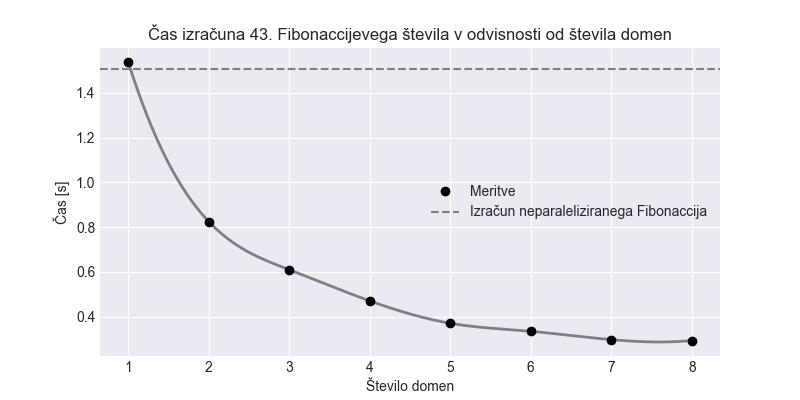
\includegraphics[width=13cm]{slike/fib_par_v_odvisnosti_od_domen.jpg}
  \label{fig:fib_par_v_odvisnosti_od_domen}
\end{figure}

Vidimo, da število domen vpliva na hitrost izračuna: Z večanjem števila domen se čas izračuna Fibonaccijevega števila
zmanjšuje, kar bi za paraleliziran računalniški program tudi pričakovali. Vendar pa se čas izračuna Fibonaccijevega
števila ne zmanjšuje linearno z večanjem števila domen, temveč sprva relativno hitro, nato pa se čas izračuna pri $14.$
domeni ustali tam nekje pri treh četrtinkah sekunde. Seveda se to razlikuje od tega, na kako močnem računalniku
program poganjamo, vendar pa bi pričakovali, da je razmerje časov izračuna Fibonaccijevih števil pri pri sekvenčnem
ter paralelnem programu podobno na vseh računalnikih. Omenil bi, da sem dane izračune poganjal na osemjedrnem Applovem
MacBooku Air M1. 

Vseeno - opomniti gre, da je točno tak eksperiment točno s takimi rezultati praktično nemogoče replicirati.
Že samo s tem, da sem prvič program poganjal medtem ko sem imel odprte še tri druge aplikacije, 
drugič pa samo medtem ko sem imel odprt zgolj naš program, sem v drugem primeru dobil skoraj dvakrat hitrejši čas izračuna.

Nato pa me je še zanimalo, kako se čas izračuna Fibonaccijevih števil spreminja v odvisnosti od zahtevanega
Fibonaccijevega števila ter kako se pri tem razlikuje čas izračuna med paralelnim in neparalelnim programom.
Kot že rečeno, sem empirično ugotovil, da se neparalelni program začne zatikati pri računanju Fibonaccijevih števil
večjih od $38$, zato sem tako za paralelni kot neparalelni program izračunal čase izračuna Fibonaccijevih števil od $38.$
do vključno $45.$ števila, pri čemer sem za paralelne izračune povsod uporabil $8$ domen. Dodatno sem pri tem grafu
analiziral še, kako se čas izračuna Fibonaccijevih števil spreminja z nižanjem praga sekvečnosti (prag fibonaccijevega,
kjer paralelni program nehamo računati paralelno, temveč sekvenčno). Zanimalo me je še, kako se čas izračuna
Fibonaccijevih spreminja, če prag sekvenčnosti zmanjšamo. V našem primeru sem tako izbral dva praga sekvenčnosti:
$35$ in $38$. Rezultati so prikazani na sliki \ref{fig:fib_par_v_odvisnosti_od_n}.

\begin{figure}[h!]
  \centering
  \caption{Čas izračuna Fibonaccijevih števil v odvisnosti od zahtevanega Fibonaccijevega števila: Paralelno in neparalelno}
  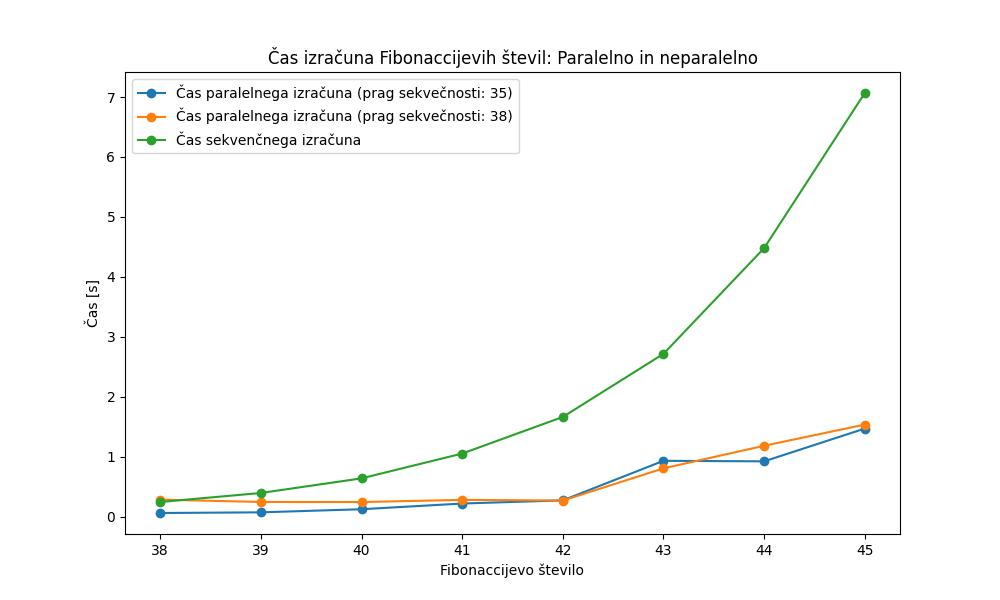
\includegraphics[width=15cm]{slike/fib_par_v_odvisnosti_od_n.jpg}
  \label{fig:fib_par_v_odvisnosti_od_n}
\end{figure}

Vidimo, da se čas izračuna Fibonaccijevih števil pri paralelnem programu z večanjem zahtevanega Fibonaccijevega števila
povečuje počasneje kot pri sekvenčnem programu. Pri neparalelnem programu se čas izvajanja, kot bi
si mislili, povečuje eksponentno (saj je časovna zahtevnost računanja eksponentna), pri paralelnem programu pa se čas
izvajanja povečuje počasneje.

\subsection{Paralelno iskanje v širino (PBFS)}

BFS rešuje širok nabor problemov, kot so na primer: Raziskovanje grafa, iskanje najkrajše poti v neuteženem grafu, 
ugotavljanja, če med dvema vozliščema obstaja pot, ugotavljanje, če je graf dvodelen, prav tako pa predstavlja osnovo
za kompleksejše grafovske algoritme, npr. za Dijkstro.

Pri predmetih iz drugega in tretjega letnika (OR, PSA1) smo se naučili, da BFS deluje tako, da vozlišča razvršča
v vrsto, nato pa iz vrste izbira vozlišča, ki jih bo raziskal, nato pa to induktivno ponavlja za vse sosede.

Ideja sekvenčnega algoritma je preprosta: Vozlišča, ki jih je potrebno raziskati, hranimo v vrsti. Na vsakem koraku
iz vrste vzamemo vozlišče, ki ga bomo raziskali, nato pa v vrsto dodamo vse njegove sosede, ki še niso bili obiskani.
Ta postopek ponavljamo, dokler ne pridemo do vozlišča, ki ga ne moremo raziskati, saj nima neobiskanih sosedov.
Paralelna verzija tega algoritma je nekoliko bolj zapletena. Pri ideji implementacije algoritma mi je najbolj pomagala
literatura \cite{spaa2010}.

\subsubsection{Sekvenčni BFS}

Ker je rekurzija elementarno orodje v funkcijskih jezikih, sem se sekvenčne implementacije BFS lotil rekurzivno, kar
je za iskanje v širino mogoče bolj redko kot iterativna verzija tega algoritma. 

Ideja je, da na vsakem koraku dodamo množico vseh dosegljivih vozlišč iz trenutnega nivoja. To lahko naredimo tako, da
za vsako vozlišče $u$ na trenutnem nivoju $L$ dodamo v množico $L$ vse njegove sosede, ki še niso bili obiskani.

Tu je moja implementirana sekvenčna implementacija tega algoritma:

\begin{lstlisting}[label=lst:bfs_sequential]
module BfsAlgorithms : Bfs = struct
  let visit_node (node : Node.t) (visited : NodeSet.t)
      (graph : UnweightedGraph.t) : Node.t list =
    let neighbours : Node.t list = 
      UnweightedGraph.neighbours node graph in
    List.filter (
      fun node -> not (NodeSet.mem node visited)) neighbours

  let rec loop (visited : NodeSet.t) 
      (stages : NodeSet.t list)
      next_stage_implementation
      (graph : UnweightedGraph.t) : NodeSet.t list =
    match stages with
    | last_stage :: _ ->
        let next : NodeSet.t =
          next_stage_implementation visited last_stage graph
        in
        if NodeSet.is_empty next then List.rev stages
        else
          loop
            (NodeSet.union visited next)
            (next :: stages) next_stage_implementation graph
    | [] -> failwith "Should not happen"

  let sequential graph start_node : NodeSet.t list =
    let next_stage_seq visited previous_stage
        (graph : UnweightedGraph.t) : NodeSet.t =
      let new_nodes : Node.t list =
        previous_stage |> NodeSet.elements
        |> List.map (
          fun node -> visit_node node visited graph)
        |> List.flatten
      in
      List.fold_left
        (fun set node -> NodeSet.add node set)
        NodeSet.empty new_nodes
    in
    loop
      (NodeSet.singleton start_node)
      [ NodeSet.singleton start_node ]
      next_stage_seq graph
end

\end{lstlisting}


Implementacijsko to počnem preko funkcije \texttt{loop}, ki na vsakem koraku dodaja nove nivoje v seznam nivojev.
Funkcija \texttt{loop} sprejme množico obiskanih vozlišč, seznam nivojev, funkcijo, ki določa, kako se izračuna
naslednji nivo, ter graf, v katerem iščemo. Funkcija \texttt{loop} na vsakem koraku izračuna naslednji nivo, nato pa
rekurzivno kliče samo sebe, dokler ne pride do nivoja, ki ne vsebuje nobenega vozlišča. Takrat vrne seznam nivojev.

Funkcija \texttt{sequential} je zgolj vmesna funkcija, ki kliče funkcijo \texttt{loop} z ustrezno funkcijo, ki
izračuna naslednji nivo. V tem primeru je to funkcija \texttt{next\_stage\_seq}, ki za vsako vozlišče na trenutnem
nivoju izračuna njegove sosede, ki še niso bili obiskani. To pa stori preko matematične funkcije \texttt{map}, ki
na seznamu vozlišč iz trenutnega nivoja kliče metodo \texttt{visit\_node}, ki za dano vozlišče izračuna njegove
sosede, ki še niso bili obiskani. Nato pa vse te sosede združi v eno samo množico, ki jo vrne.

\subsubsection{Paralelni BFS}

Namerno sem v \ref{lst:bfs_sequential} metodo \texttt{sequential} napisal modularno, tako da lahko paralelizacijo
dodamo zgolj z zamenjavo funkcije \texttt{next\_stage\_seq} z ustrezno funkcijo, ki bo izračunala naslednji nivo
paralelno. To sem naredil v metodi \texttt{parallel}.

\begin{lstlisting}[label=lst:bfs_parallel]
module BfsAlgorithms : Bfs = struct
  ...

  let parallel graph start_node
      ~(num_domains : int) : NodeSet.t list =
    let next_stage_par visited previous_stage graph =
      let new_nodes : Node.t list =
        previous_stage |> NodeSet.elements
        |> Parmap.parmap num_domains (
          fun node -> visit_node node visited graph)
        |> List.flatten
      in
      List.fold_left
        (fun set node -> NodeSet.add node set)
        NodeSet.empty new_nodes
    in
    loop
      (NodeSet.singleton start_node)
      [ NodeSet.singleton start_node ]
      next_stage_par graph

  ...
end

\end{lstlisting}

Če smo prej preko metode \texttt{map} za vsako vozlišče na trenutnem nivoju izračunali njegove sosede sekvenčno,
je tu ideja paralelizacije v tem, da to naredimo vzporedno. Našel sem knjižnico \texttt{Parmap}, ki nam omogoča
paralelizacijo metode map na seznamu. Ta knjižnica je zelo preprosta za uporabo, saj je potrebno zgolj zamenjati
funkcijo \texttt{map} z \texttt{parmap} in dodati še število domen, ki jih želimo uporabiti. Knjižnica sama poskrbi
za vse ostalo.

\subsubsection{Analiza časa računanja BFS algoritmov}

V tem razdelku bom analiziral časovno zahtevnost paralelnega BFS algoritma v primerjavi s sekvenčnim.
Za razliko od pohitritve algoritma računanja Fibonaccijevih števil, kjer je paralelno računanje pospešilo naš proces,
se je pri paralelnem BFS algoritmu izkazalo, da je paralelno računanje celo upočasnilo naš proces. Vseeno
pa tu predstavim rezultate ter povzamem, kako sem se merjenja časa računanja grafov lotil empirično.

Vemo, da je časovna kompleksnost sekvenčnega BFS algoritma $O(|V| + |E|)$, kjer je $|V|$ število vozlišč v grafu,
$|E|$ pa število povezav v grafu, zato je pričakovati, da bo čas izračuna sekvenčnega BFS algoritma naraščala linearno
z velikostjo grafa. Da sem lahko primerjal časa izračuna sekvenčnega in paralelnega algoritma, sem izračunal ustvaril
$16$ grafov, ki so po številu svojih vozlišč in povezav linearno naraščali, pri čemer je imel največji graf
$2000$ vozlišč ter $1000000$ povezav. Na sliki \ref{fig:bfs_calculation_time_by_graph_size} so predstavljeni izmerjeni
rezultati.

\begin{figure}[h!]
  \centering
  \caption{Čas izračuna BFS algoritma v odvisnosti od števila vozlišč ter povezav}
  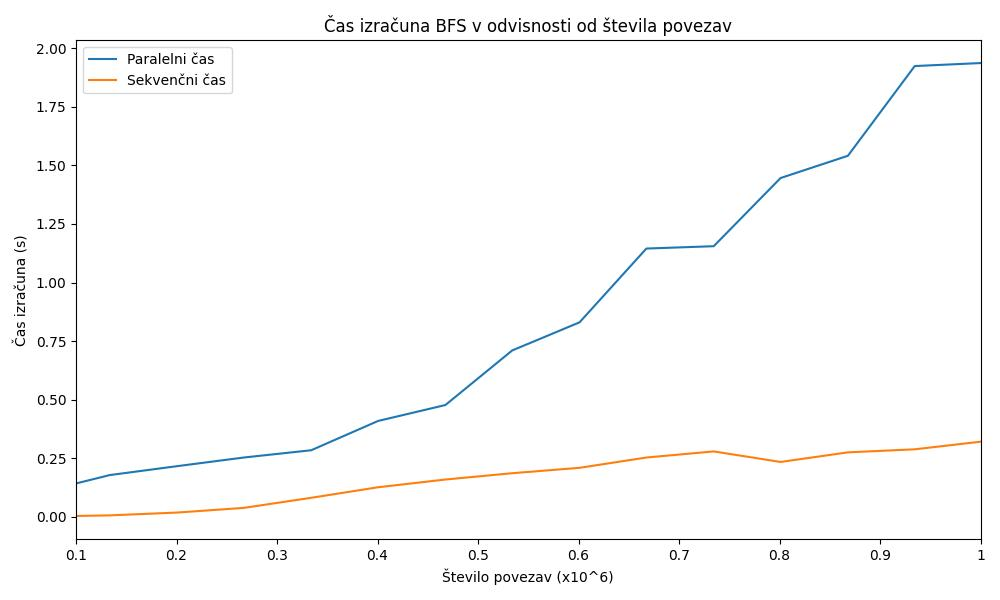
\includegraphics[width=15cm]{slike/bfs_v_odvisnosti_od_velikosti_grafa.jpg}
  \label{fig:bfs_calculation_time_by_graph_size}
\end{figure}

Čeprav tudi čas izračuna paralelnega algoritma narašča linearno z velikostjo grafa, je vseeno precej počasnejši od
sekvenčnega algoritma. Po večih poskusih optimizacije paralelnega algoritma nisem našel algoritma, ki bi bil pri
večino grafih hitrejši kot sekvenčni, razlogov pa je lahko več:
\begin{itemize}
  \item \textbf{Dodatna računaska obremenitev zaradi paralelizacije: } Paralelizacija algoritma zahteva dodatne operacije, kot so 
        razdeljevanje dela med niti, sinhronizacija med nitmi in pošiljanje rezultatov nazaj v glavni program. 
        Vse te operacije lahko povzročijo dodatno računsko obremenitev (overhead), ki upočasni izvajanje algoritma.
  \item \textbf{Počasnost knjižnice Parany: } Knjižnica Parany prav tako podpira samo paralelizacijo na nivoju
        procesorja, kar je lahko precej počasneje kot paralelizacija na nivoju pomnilnika za dano metodo. Prav tako
        pa je bila ta knjižnica napisana več let nazaj ter posledično ni ustvarjena za OCaml 5 ter najnovejše
        procesorske arhitekture.
  \item \textbf{Naivna paralelizacija: } V zgornji kodi sem paraleliziral vsak funkcijski klic. Ideja, ki mi je zaradi
        premajhnega obsega diplomske naloge ni uspelo implementirati je, da bi na neki točki avtomatsko ugotovil,
        kateri deli kode so najbolj računsko zahtevni, ter te dele kode paraleliziral, druge pa bi pustil, da se
        računajo na enem samem jedru.
\end{itemize}

Dodatno me je zanimalo še, kako se čas izračuna paralelnega BFS algoritma spreminja z večanjem števila domen.
Zato sem si izbral graf z $500000$ povezavami, ter ga računal paralelno z različnim številom domen. Rezultati so
prikazani na sliki \ref{fig:bfs_calculation_time_by_num_domains}.

\begin{figure}[h!]
  \centering
  \caption{Čas izračuna paralelnega BFS algoritma v odvisnosti od števila domen}
  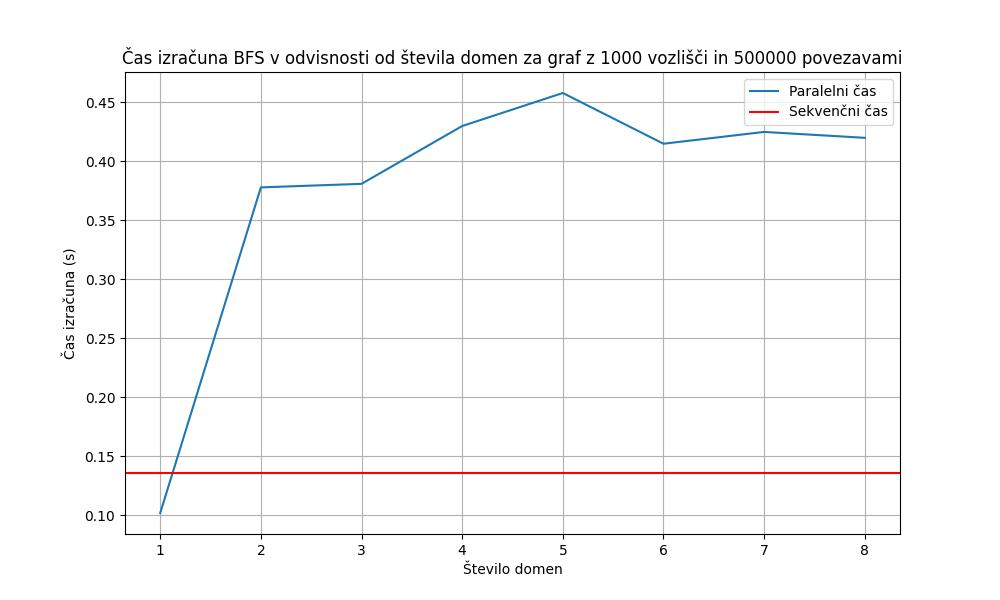
\includegraphics[width=15cm]{slike/bfs_v_odvisnosti_od_stevila_domen.jpg}
  \label{fig:bfs_calculation_time_by_graph_size}
\end{figure}

Vidimo lahko, da je paralelni algoritem spet počasnejši od sekvenčnega - pri eni domeni je seveda z sekvenčnim primerljiv,
pri več kot eni domeni pa je počasnejši, kar prav tako potrjuje hipotezo, da je je paralelizacija algoritma za iskanje
v širino na nivoju procesorja počasnejša od svojega sekvenčnega ekvivalenta.


\subsection{Paralelna implementacija Dijkstrovega algoritma} \label{section:dijkstra}

TODO.



\end{document}
